\documentclass{sig-alternate-05-2015}
\makeatletter
\def\@copyrightspace{\relax}
\makeatother
\begin{document}

% Copyright
\setcopyright{acmcopyright}

\title{Web Economics: Group 09 Report}

\numberofauthors{3}
\author{
\alignauthor
Devin Kuokka\\
       \affaddr{Affiliate Student, Computer Science, University College London}\\
       \email{devin.kuokka.16@ucl.ac.uk}
\alignauthor
Stylianos Rousoglou\\
       \affaddr{Affiliate Student, Computer Science, University College London}\\
       \email{stylianos.rousoglou.16
       @ucl.ac.uk}
\alignauthor
Michael Whitman\\
       \affaddr{Affiliate Student, Computer Science, University College London}\\
       \email{zcabwhi@ucl.ac.uk}
}
\maketitle

\section{Introduction}
Real-Time Bidding (RTB) is an increasingly popular approach to online advertising that has evolved into a multi-billion dollar industry. An efficient approach to quickly and accurately optimizing an advertiser's bidding strategy in ad auctions is paramount to the success of the advertising party, as a good solution can save vast amounts of money and lead to higher conversion rates than competitors.

The challenge in automating ad auctions and bidding in real-time is the necessity to predict, with the highest possible accuracy, the likelihood that the ads displayed to a particular user will actually be of interest to them. Using those predictions, hereby referred to as pCTR (or predicted Click-Through Rate), a strategy can be developed to optimize the number of won impressions (which the advertiser pays for) that have the potential of becoming conversions. Naturally, the accuracy and sensitivity of the pCTR values in central in developing a successful bidding strategy.

Given real-life ad impression data, a machine learning approach is often preferred in tackling this problem. First, a large data set with \textit{training} data is used to build and optimize some type of machine learning classifier. After the machine learning model is trained, it is used to make predictions about data in a \textit{test} data set, for which user feedback is not provided, thus attempting to predict unknown users' behavior. The success of the classifier is evaluated by different metrics that reflect its accuracy in anticipating an unknown user's responsiveness to an ad. The machine learning approach undertaken in my personal strategy is \textit{logistic regression}.

Therefore, in attempting to predict user behavior, a thorough and educated study and use of the training data is required for accurate and useful results. Our individual reports present some data analytics that result from a basic exploration of the training data set provided for the assignment. 

In this paper, different approaches to automating the generation of bid prices will be undertaken, and each will be evaluated using common evaluation metrics and comparatively to others. First, two naive strategies with little optimisation will be implemented, and the results will be presented and discussed. Subsequently, two machine learning approaches will be presented, one using a linear model and one using a non-linear one. Our approach and steps in building our machine learning classifier and developing a bidding strategy will be detailed. The techniques employed throughout our group strategies will be discussed, and different design decisions made will be defended. Finally, the results of our best strategy will be presented and commented on using relevant evaluation metrics.

\section{Related Work}
The extensive literature review we performed covers a range of academic papers and articles. The first academic paper, \textit{Real-time bidding benchmarking with ipinyou dataset}, was used as a model for both the presentation of the data and the preliminary statistical analysis performed on the dataset, both to be found in our individual reports. The second relevant publication, \textit{A logistic Regression Approach to Ad Click Prediction}, provided valuable insights into building a logistic regression classifier, which is the machine learning model used in our group solution, as well as into techniques for data pre-processing, data clensing and data reduction. Other related work submitted in the past 5 years to KDD (Knowledge Discovery and Data Mining), a community producing scientific work in data mining and data analysis, was also reviewed for additional observations and expertise.

\section{Dataset}
The dataset consists of three data files, namely the training, validation, and test files. Machine learning classifiers are first trained using the training data set, \textit{train.csv}. Subsequently, the \textit{validation.csv} file is used to evaluate the performance of different classifiers and suggest which algorithm is more accurate in its predictions. While the aforementioned files include user feedback information about each ad impression, which is necessary for supervised learning as it is used to train, optimize and evaluate the classifier (in the case of RTB, user feedback refers to whether the ad was clicked or not, i.e. a binary variable), the third file, \textit{test.csv}, is only used for testing the developed model, and thus does not contain the \textit{click} data field. Auction pricing information is also not included in the testing dataset, as the solution is required to optimize bidding prices and come up with the best possible strategy to win as many likely-to-be-clicked impression auctions as possible, thus maximizing the conversion rate of ad impressions.

\subsection{Data format}
The dataset includes thousands of impressions, one per line, in comma-separated csv files, with detailed information about the advertiser, the advertising context, the spatial and temporal context, and the user, for each impression. The format of the data varies across fields, with integers, strings, as well as special words and symbols used. In instances where data is missing, the word \textit{null} is used. Fields such as \textit{weekday} and \textit{hour} have been mapped to integers, while others, such as \textit{useragent}, have been left as string. It is clear that some data manipulation has to be performed prior to the data beind used for training a classification model.

Note that, although the dataset uses the currency RMB and units of Fen x 1000 in all figures pertaining to money, all monetary results in this report (such as cost, effective CPC, etc.) have been adjusted to units of Fen.

\section{Approach \& Evaluation}
There were several non-trivial approaches our group experimented with, including linear and non-linear solutions. Below, the constant and random bidding strategies are first discussed, and then a linear and a non-linear approach are presented.

Python was used for developing the main functionality of all the solutions and learning algorithms, as well as for common helper code used for loading the data, storing the output in a convenient format, and displaying a summary of the results in the terminal. The \textit{scikit-learn} \footnote{http://scikit-learn.org} Python library was used for the actual logistic regression functionality. Other Python libraries, such as \textit{pandas}\footnote{http://pandas.pydata.org/}, a data analysis software library, and \textit{numpy}\footnote{http://www.numpy.org/}, a scientific computing software package, were also utilized to facilitate data analysis and manipulation.

\subsection{Basic Strategies}

\begin{figure}
  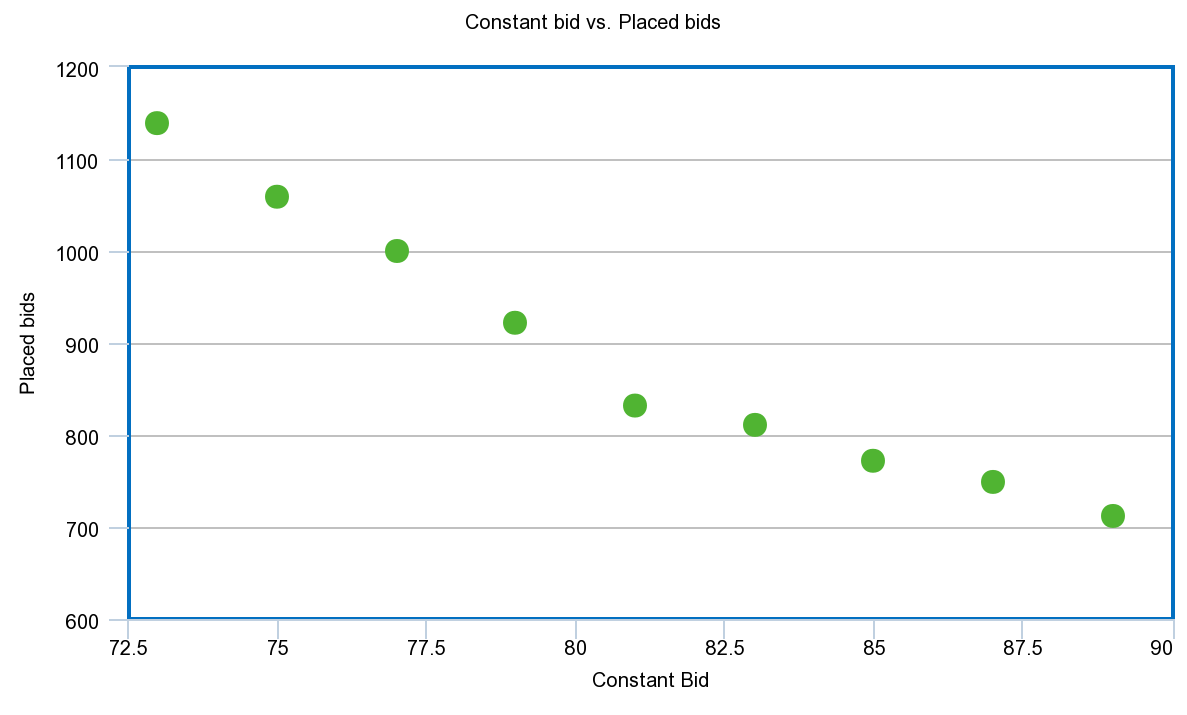
\includegraphics[width=\linewidth]{Bids.png}
  \caption{Constant bid vs. Placed bids}
  \label{fig:bids}
\end{figure}

\begin{figure}
  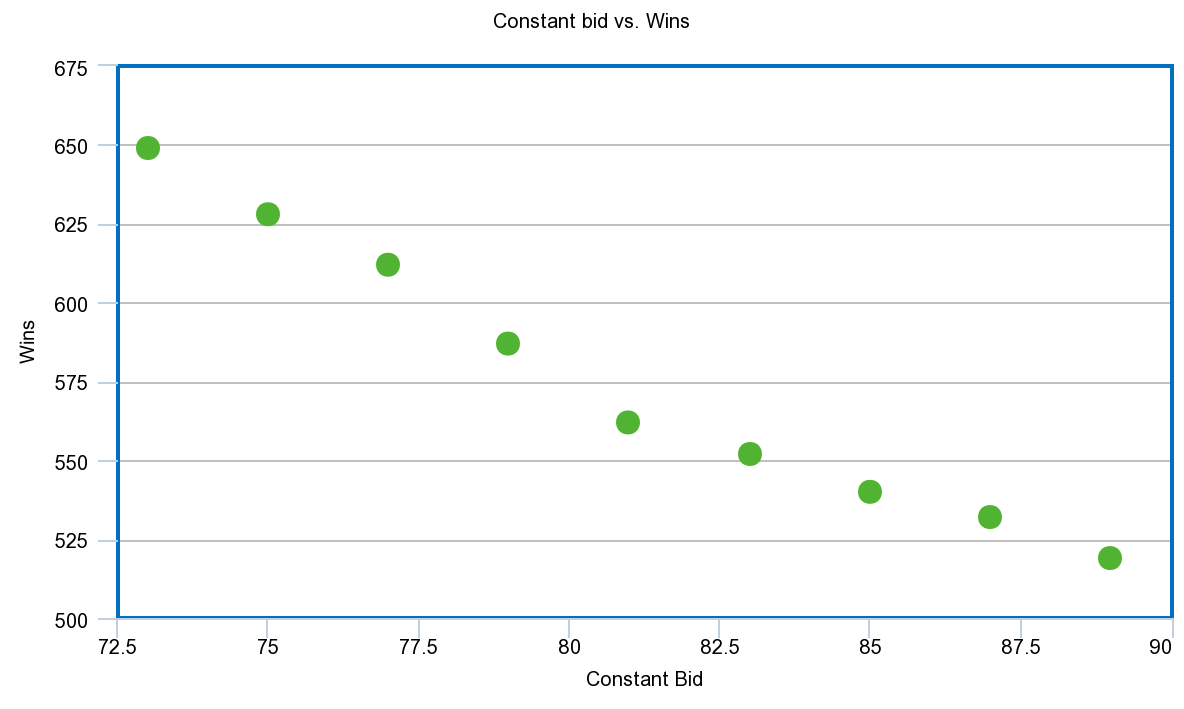
\includegraphics[width=\linewidth]{wins.png}
  \caption{Constant bid vs. Wins}
  \label{fig:wins}
\end{figure}

\begin{figure}{h}
  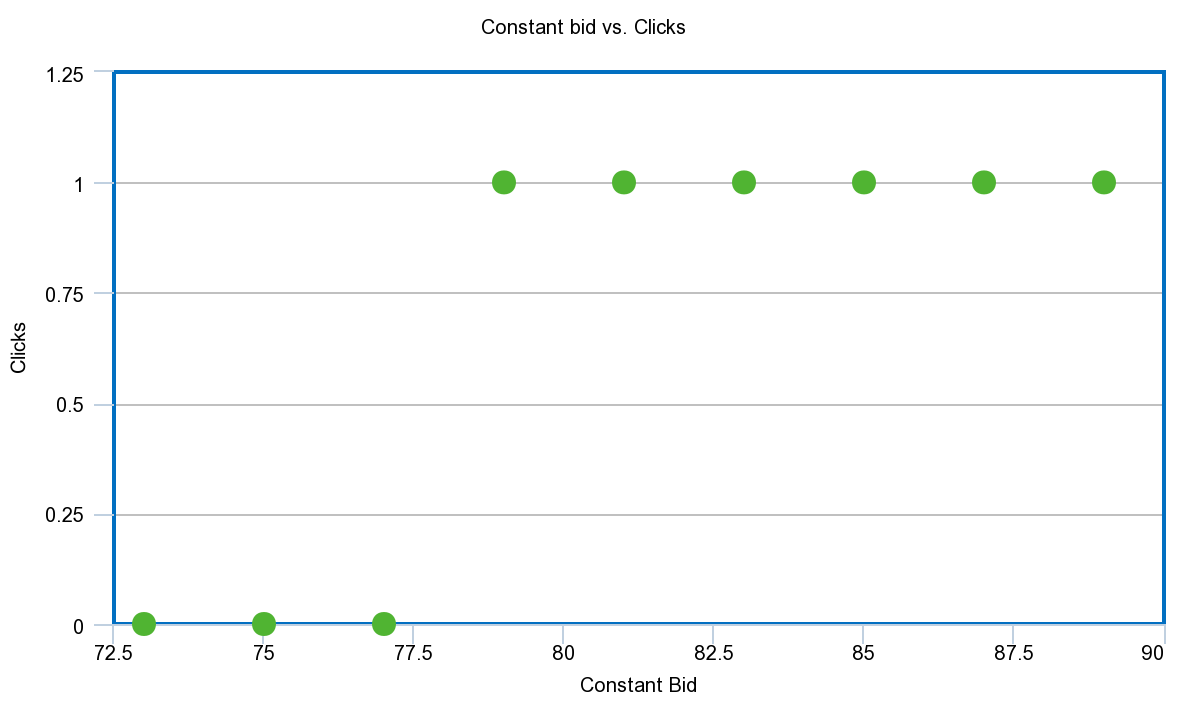
\includegraphics[width=\linewidth]{click.png}
  \caption{Constant bid vs. Clicks}
  \label{fig:clicks}
\end{figure}

\begin{figure}{h}
  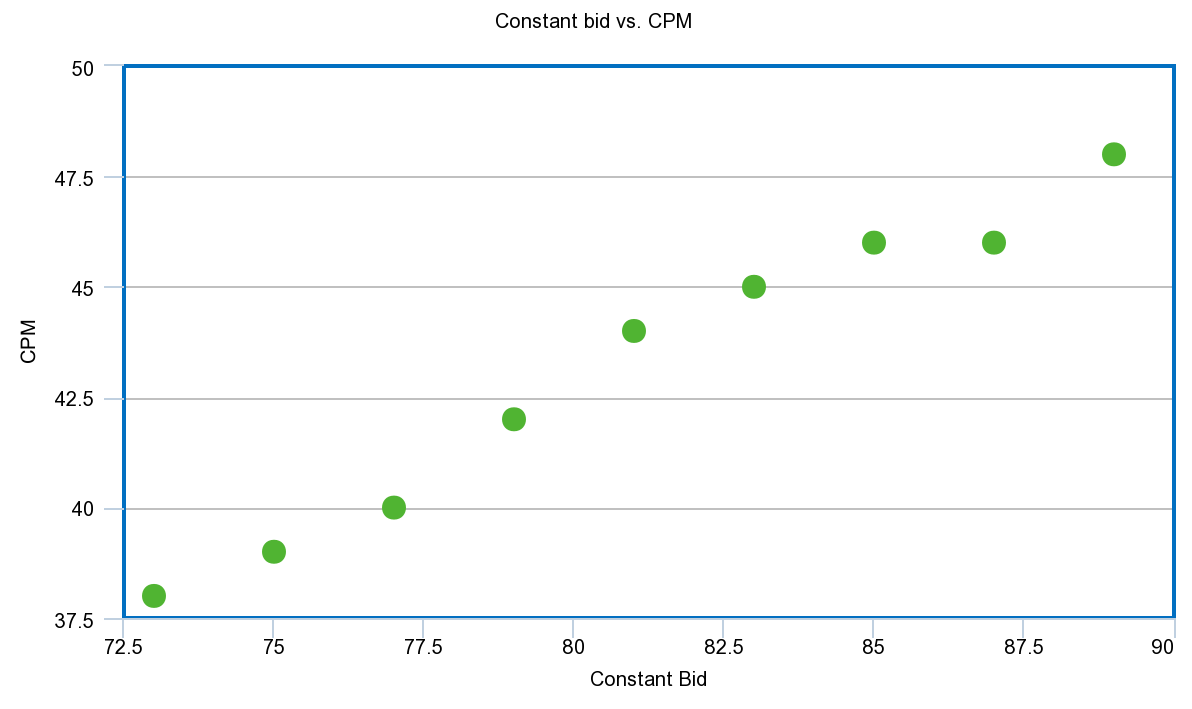
\includegraphics[width=\linewidth]{CPM.png}
  \caption{Constant bid vs. CPM}
  \label{fig:CPM}
\end{figure}

\subsubsection{Constant Bid}
The first strategy was a rather simple one; the solution had to bid the same constant value in every auction. Given the budget constraint of $25,000$, the task can be treated as an optimization problem with the following limiting cases: the algorithm's bids are too high, which results to all auctions being won and the budget rapidly running out; or the algorithm's bids are too low, which results to too few auctions being won and the budget not being spent. 

Clearly, the optimal solution lies somewhere in between the two limiting cases. This approach would in theory help us win more bids than choosing a constant bid by chance, and assuming that impressions that will be clicked are uniformly distributed in the dataset, it also increases the expected CTR, since the budget will all be spent, but not immediately and on consecutive bids. Therefore, we proceeded to calculating the \textit{mean} payprice in the training dataset and using that to define a range of values that we would explore. To approximate the optimal constant bidding amount, we plotted that range of probable values around the mean against several evaluation metrics, with the results presented above. 

Figures 1 and 2 show the constant bid value plotted against the bids placed and the bids won by the solution respectively. The results are perfectly consistent with the notion that a high constant bid value places less bids and wins less auctions that a lower one. Additionally, the fact that significant differences in bids and wins are observed for slight variations of the constant bid suggests that the payprice values in the dataset are concentrated around the mean value (which is around 80).

Figure 3 plots the bid value against the number of clicked impressions. As expected, the Constant Bid solution is performing very poorly, and the Click results are not of much insterest since we only see values of one or no clicks at all, which offers no valuable insights on how CTR varies with those changes in the constant bid. For the data points of 1 click, we can conclude that the solution starts consistently winning one patricular auction that leads to a conversion, the price of which is over 77.3, or approximately 79.

Figure 4 shows the bid value against the Cost per million impressions, which expectedly increases since a higher constant bid implies more expensive auctions being won, and thus more money being spent per million impressions.

The CTR is $0\%$ for runs where no impressions were clicked, and about $0.00033\%$ for the latter runs with one clicked impression. This CTR is significantly low, considering that the percentage of clicked impressions in the training dataset is more than 100 times greater, specifically about $0.077\%$.

\subsubsection{Random Bid}

\begin{figure}
  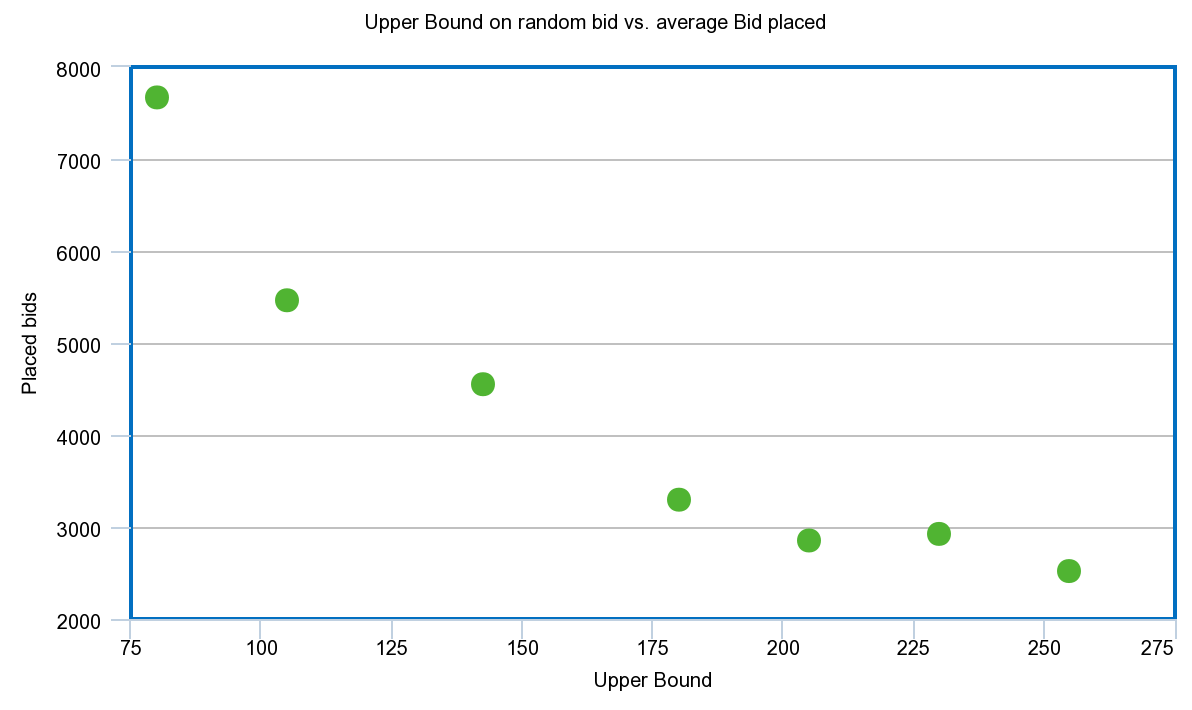
\includegraphics[width=\linewidth]{random_bids.png}
  \caption{Upper bound vs. Placed bids}
  \label{fig:bids}
\end{figure}

\begin{figure}
  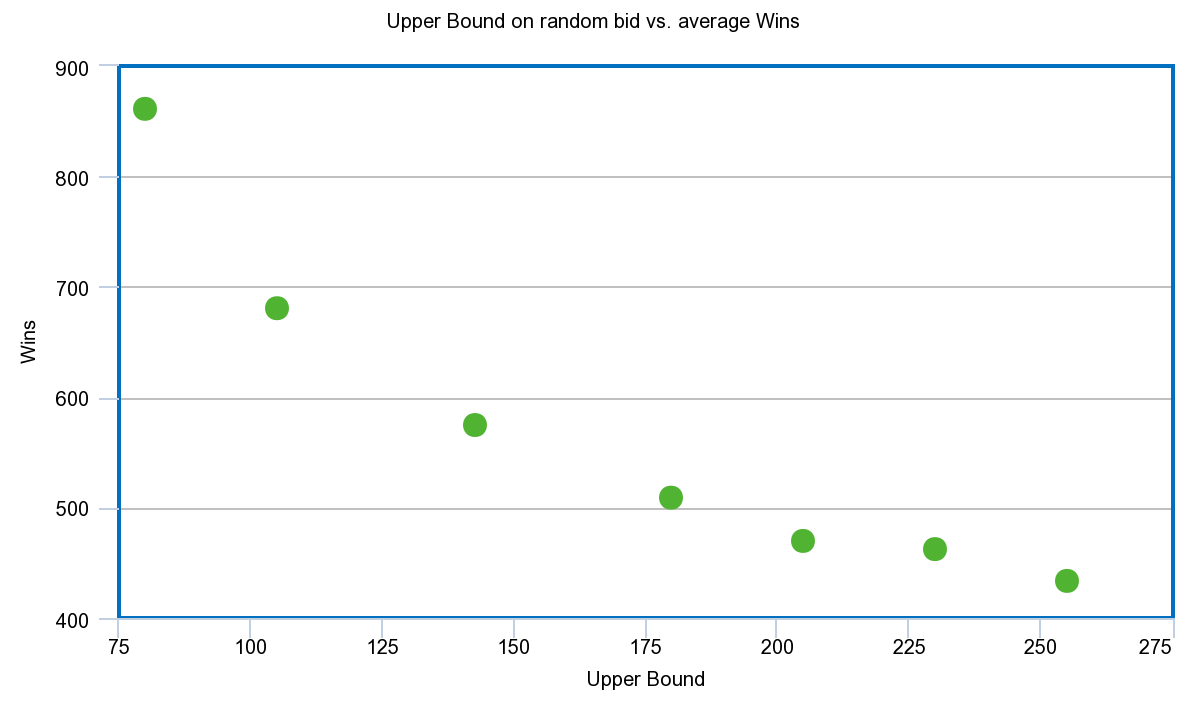
\includegraphics[width=\linewidth]{random_wins.png}
  \caption{Upper bound vs. Wins}
  \label{fig:wins}
\end{figure}

\begin{figure}
  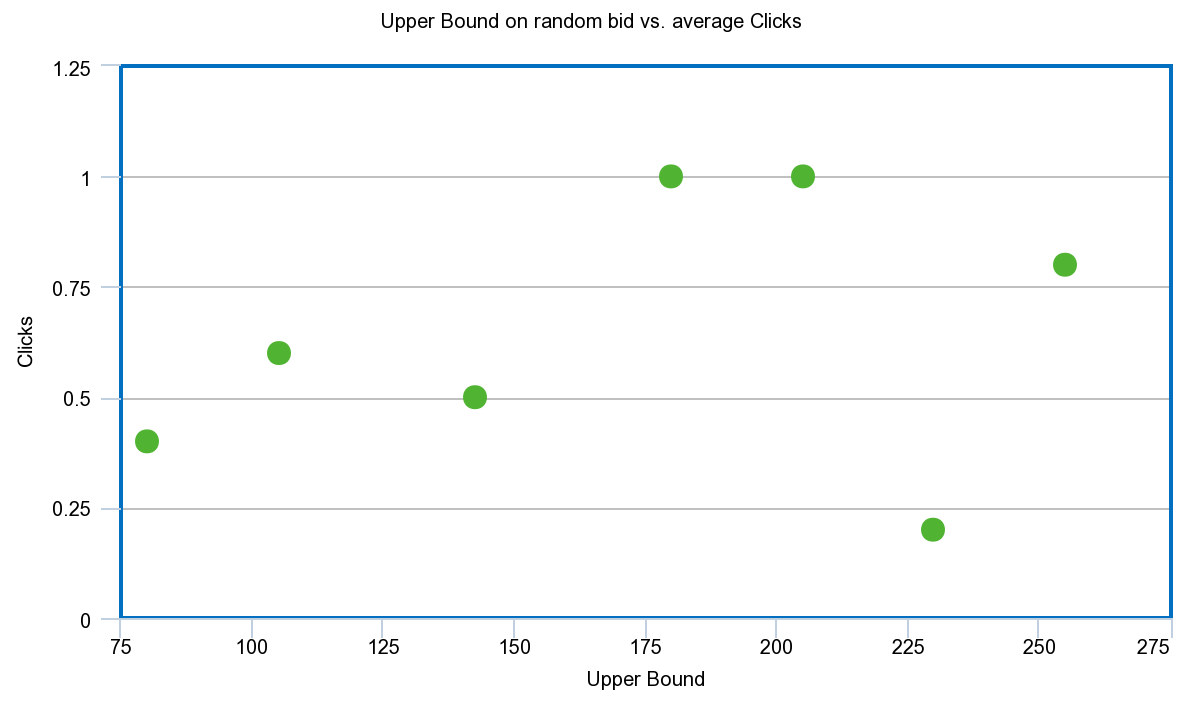
\includegraphics[width=\linewidth]{random_clicks.png}
  \caption{Upper bound vs. Clicks}
  \label{fig:clicks}
\end{figure}

\begin{figure}
  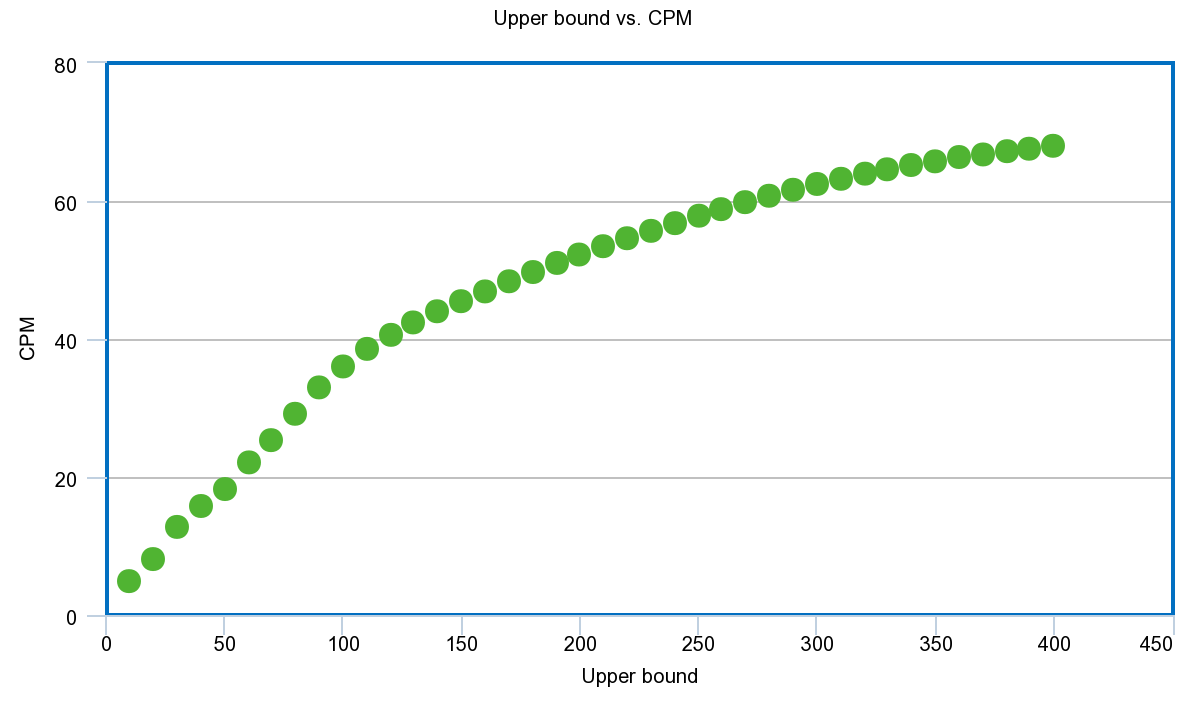
\includegraphics[width=\linewidth]{random_CPM.png}
  \caption{Upper bound vs. CPM}
  \label{fig:CPM}
\end{figure}

The second simple strategy we explored introduced randomness in the strategy's bidding choices by basing the bid prices on chance. Our approach in exploring a range of possible upper bounds was the following: after calculating the mean impression pay price from the training dataset, we created a range of values by adding fractions of the standard deviation to the mean. To make our results more reliable, we ran the evaluation process on validation.csv \textit{five times} for each value in the explored upper bound range. The vertical axes then plot the \textit{average} values obtained from five distinct trials with each given upper bound.

To enforce the upper bounds, we used a Python function to generate pseudo-random numbers in the range $[0,1]$, and then multiplied them by our upper bounds, thus getting a series of pseudo-randomly generated real values in the range $[0, UpperBound]$.

Figures 5 and 6 show the number of placed bids and wins respectively, as a function of the upper bound fed into our pseudo-random number generator. As expected, increasing the upper bound of the random bids leads to an increase in the expected average number of bids placed. Therefore, the trend observed is similar to that of Figure 1, where the actual average number of bids was inveresely proportional to the value of the constant bid.

Figure 7, which plots the upper bound against the number of clicked impressions, reveals why a random-based approach to solving the problem is bound to not perform reliably well. Although repeating the experiment infinite times would give expected values that follow a certain increasing trend, five trials were clearly not enough to demonstrate any consistent trend or correlation between the two values. Since the bidding values are randomly chosen, there is no guarantee on the performance of the solution on any given run.

Figure 8 plots the solution's CPM as a function of the upper bound of our pseudo-randomly generated bid values. The trend observed is similar to the trend in Figure 4, which makes intuitive sense since increasing the expected average bid value should lead to more expensive auctions being won and paid for.

The calculated average CTR of this solution was again about $0.00033\%$, reflecting the inadequacy of this solution and its bad results, which are similar to those of the constant bid approach.

\subsection{Machine Learning Strategies}
Several regression and classification machine learning algorithms were considered by our team. The problem lends itself well for supervised learning; the training dataset does contain auction results as well as user feedback, and the goal is to build a classifier that produce a CTR estimate for any given impression. Our initial instinct was to use Linear Regression, a quite familiar and conceptually simple approach. Linear Regression uses the general linear function $y = a_0 +  \sum a_i x_i$, where the dependent variable $y$ is \textit{continuous}, as is \textit{usually} the case for the independent variables $x_i$ as well. It is tempting to use the linear model result as a probability, but there is a fundamental problem with that: the output of the linear model \textit{can be less than 0 or greater than 1}, rendering the output meaningless. 

To solve this problem, \textit{Logistic Regression} was introduced, with a mathematical model that actually restricts the dependent variable value in the range $[0,1]$. In reality, the model is estimating \textit{the probability} of a categorical outcome, i.e. the likelihood of one discrete output result versus another. The general Logistic Regression formula for two outcomes (0 or 1) can be written as \[P(Y=1) = \frac{1}{1+e^-(a_0+\sum a_i x_i)}\]
Though the independent variables may either be continuous or discrete, the result of the model is a probability of the dependent output taking the given discrete value.\footnote{https://www.quora.com/What-is-logistic-regression}

Logistic Regression was the approach finally undertaken by our group. Logistic regression is a \textit{binary classification} algorithm, which means that the result of its predictions is discrete by nature. This caters perfectly to our problem, namely deciding whether a user will click (click = 1) an ad or not (no click = 0). Also, all impression data used for learning is categorical, which is acceptable since dependent variables in Logistic Regression may be both continuous or categorical. The underlying mechanism of Logistic Regression is Maximum Likelihood Estimation (MLE), a widely used statistical model for estimating the values of parameter variables that maximize the likelihood that the output takes an observed value. 

Before training the machine learning classifiers to make CTR predictions, there was a significant amount of work to be done in order to prepare the data for "learning". First, a high-level analysis (presented in detail in our individual reports) was useful in deciding on the good data features to be used for classification, i.e. the ones that do correlate with differences in the Click-Through Rate. Accordingly, several data fields that either had unique or highly differentiated values, such as the \textit{bidid} and the \textit{userid}, would not have been useful for classification and thus had to be removed. Therefore, some \textbf{data selection} was performed to remove those fields, as well as \textit{IP} (unique to each user), \textit{logtype} (1 in this dataset), \textit{domain}, \textit{url}, \textit{urlid}, \textit{creative}, \textit{keypage}, etc.

Given the large volume of data with negative user feedback (click = 0) and the scarcity of impressions that led to conversions (click = 1), \textbf{undersampling} was also used to increase the ratio of clicked to non-clicked impressions in the training data. The small bias towards clicked impressions in training helped correct the bias in the original dataset, where only 0.077\% of all impressions were clicked.

Subsequently, the data was tranformed using a technique known as \textit{one-hot encoding}. One-hot encoding creates a vector for every possible string value any feature can possibly take, transforming the feature-value mappings chosen for learning into sparse matrices, One-hot encoding tranforms complex feature-value mappings into simple (though very large) matrices with only binary digits, a conversion which is very helpful for mathematical computations as well as more convenient for machine learning classification algorithms.

Since one-hot encoding vastly expands the feature space, we performed \textit{feature selection} to prevent long running times of our classification algorithms and avoid problems with Logistic Regression such as \textit{overfitting}. Essentially, a subset of the large feature space was chosen, which contained the \textit{best} predictor variables in terms of degree of correlation with the output pCTR. After experimenting with the number of features we'd allow, we observed the results of the solution after using 20, 40, and 60 features (in the linear bidding strategy) were extremely similar. For values above 100 features, the solution started producing inferior results. We concluded that there must be around twenty very good features for training, so we limited the selected features to 20.

After this last step, the classifier is ready to be trained. The selected feature vectors are passed into the \textit{scikit-learn} library, and a logistic regression model is built to produce CTR predictions. It's worth noting that the option 'class weight' is set to \textit{balanced}, which means that the learning weights associated with feature classes are automatically adjusted to be inveresly proportional to class frequencies in the training data.

After learning is completed, the validation dataset is loaded and some data manipulation is performed, as described above. Subsequently, the model is used to calculate CTR predictions for every impression in the validation dataset and store them in an in-memory array. The real-time bidding simulation can then be performed, and its results evaluated.

\begin{figure}
  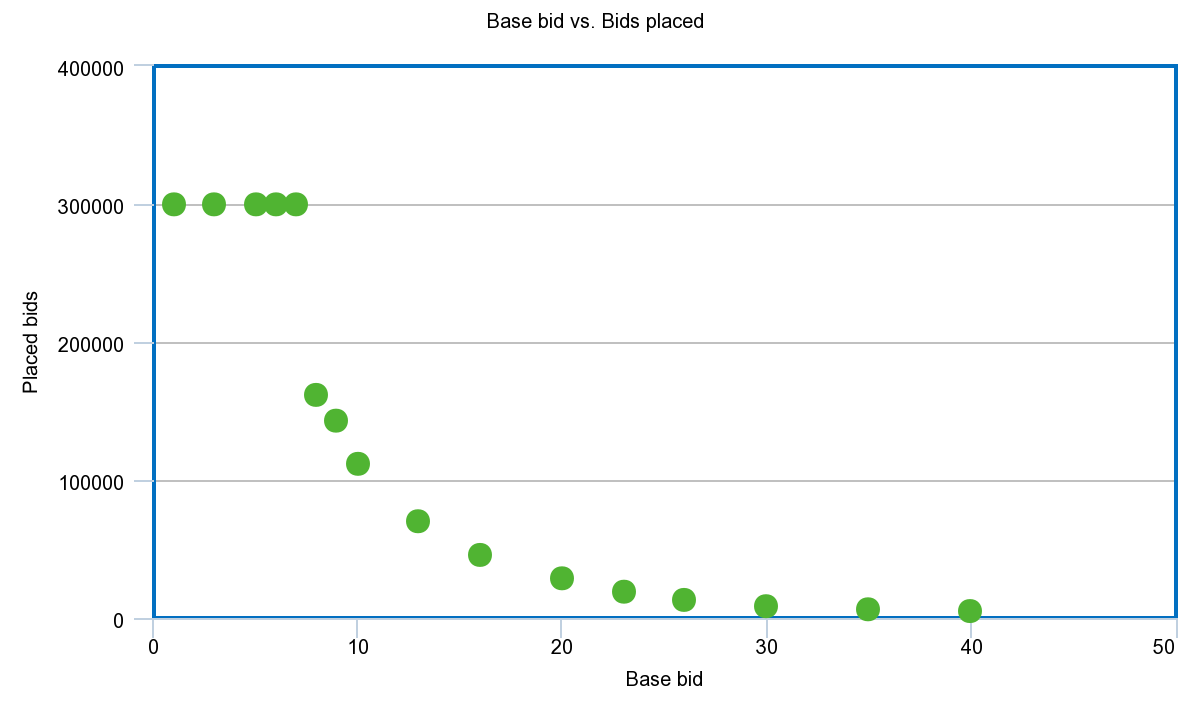
\includegraphics[width=\linewidth]{linear_bids.png}
  \caption{Base bid vs. Placed bids}
  \label{fig:bids}
\end{figure}

\begin{figure}
  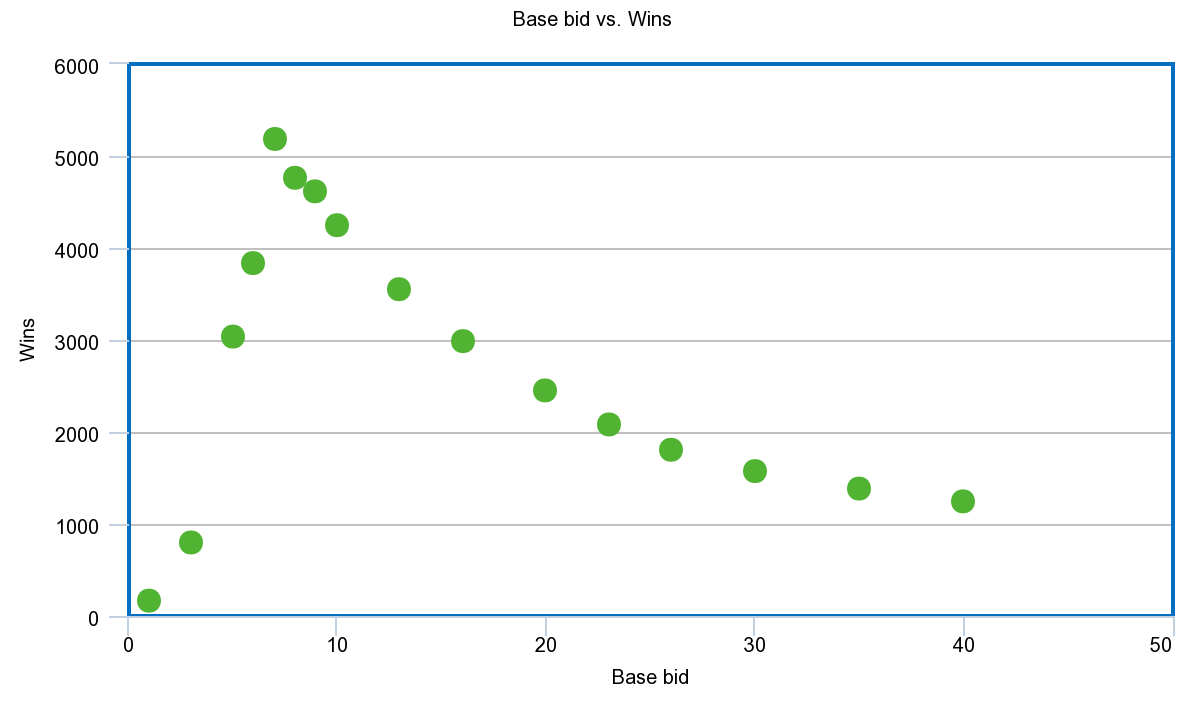
\includegraphics[width=\linewidth]{linear_wins.png}
  \caption{Base bid vs. Wins}
  \label{fig:bids}
\end{figure}

\begin{figure}
  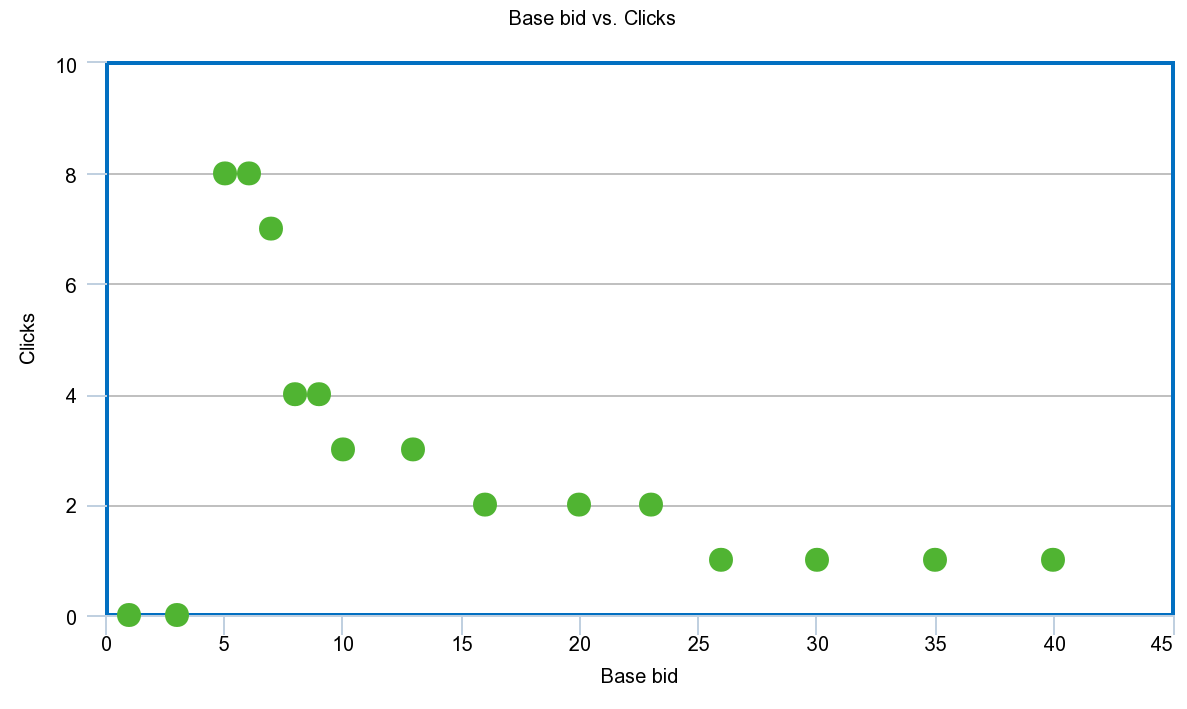
\includegraphics[width=\linewidth]{linear_clicks.png}
  \caption{Base bid vs. Clicks}
  \label{fig:bids}
\end{figure}

\begin{figure}
  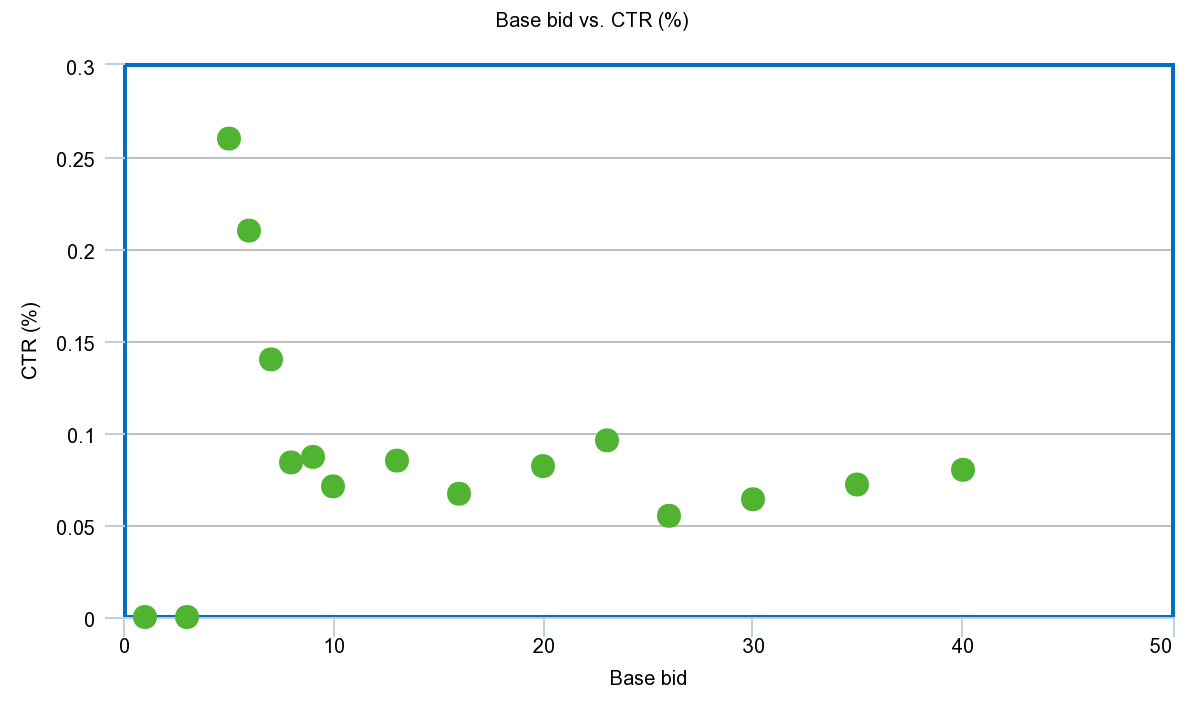
\includegraphics[width=\linewidth]{linear_CTR.png}
  \caption{Base bid vs. CTR (\%)}
  \label{fig:bids}
\end{figure}

\begin{figure}
  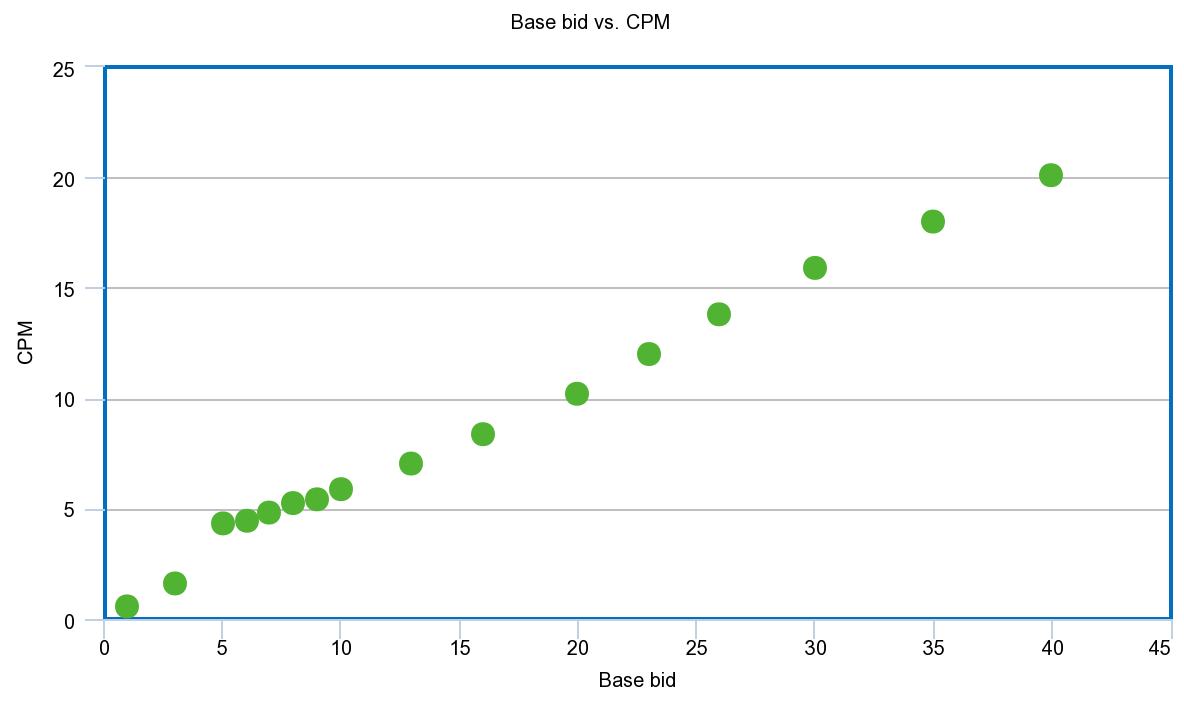
\includegraphics[width=\linewidth]{linear_CPM.png}
  \caption{Base bid vs. CPM}
  \label{fig:bids}
\end{figure}

\begin{figure}
  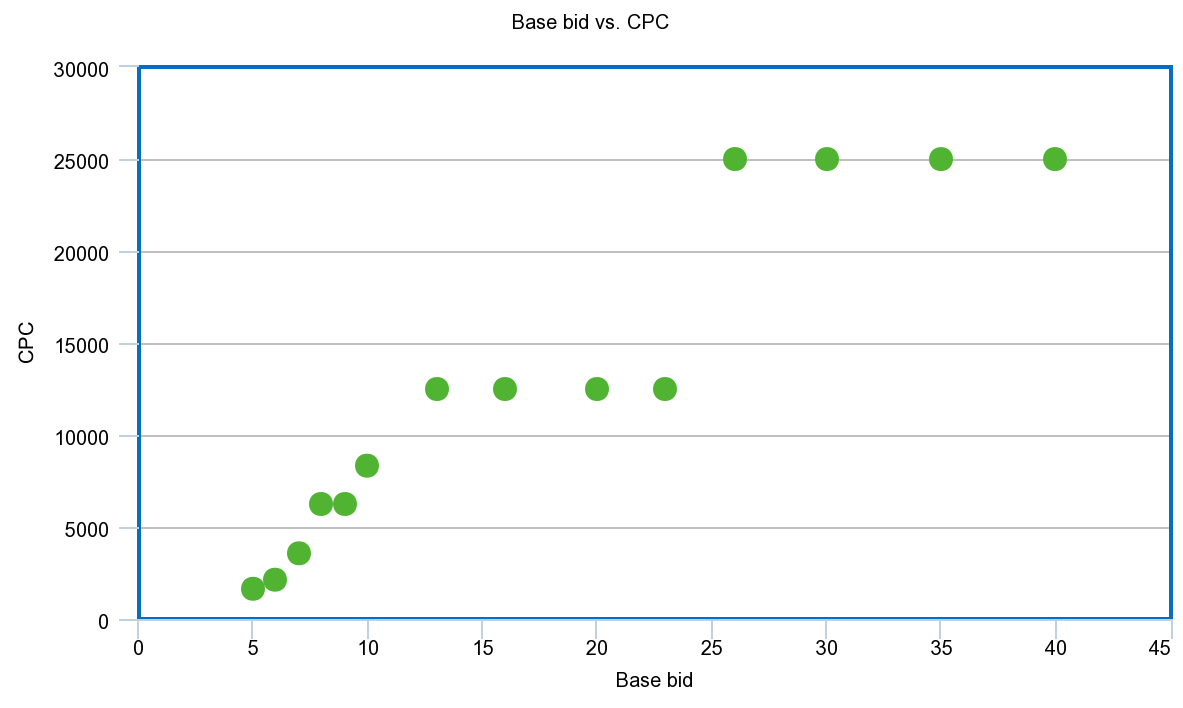
\includegraphics[width=\linewidth]{linear_CPC.png}
  \caption{Base bid vs. CPC}
  \label{fig:bids}
\end{figure}

\subsubsection{Linear Bidding Strategy}

In this linear model strategy, the bidding price for a given impression is proportional to its predicted CTR. Specifially, the formula can be written as $bid = C * (pCTR / avg CTR) $, where C is a constant that we'll refer to as the \textit{base bid}. Conceptually, the base bid would be the bid price for an impression with average CTR, i.e. for which the ratio $pCTR / avg CTR$ is $1$. For impressions with higher-than-average predicted CTR, the ratio would be over 1 and the base bid would be proportionally higher than the value of the base bid.

The first step was to calculate the mean CTR by averaging the value of the 'click' field in the training dataset. To decide on a good value for the constant \textit{base bid}, we varied the base bid value in the range $[0, 50]$ and ran the evaluation process numerous times. The results appear in Figures 9 through 14.

Figures 9 and 10 plot the base bid against the bumber of bids placed and the number of bids won respectively. The two graphs are compatible: for small base bid values, the whole budget never gets spent, s othe number of bids placed is constant and equal to the total number of impressions in the dataset, as evidence by the linear horizontal trend in Figure 9. Since the base bid is small, the corresponding range in Figure 10 shows an increasing trend in wins, as increasing the base bid leads to more percentage of the budget being spent, and thus more wins. After the threshold value of 7, where the global maximum of Figure 10 is observed,  the trend in both graphs becomes asymptotically decreasing. The whole budget is now being spent, and an increasing base bid implies more expensive - and thus less - auctions being won.

Figures 11 and 12 plot the absolute number of clicks and click-through rate percentages respectively, for the same range of base bids as figures 9 and 10. As expected, for very small base bids, no clicks are observed. Interestingly, the maximum CTR of the solution is the first non-zero data point, where $base bid = 5$. Eight conversions are achieved with the particular value, for a reasonably high CTR value of $0.263\%$, the peak of the CTR plot. The trend of figure 11 is strictly non-increasing from that point on, whereas in figure 12 several local maxima are observed. Above a base bid value of $9$, however, the CTR consistently remains under $0.1\%$.

Finally, figures 13 and 14 present money-related metrics, namely CPM and CPC as functions of the base bid. The most cost-efficient point seems to be the one with highest CTR, namely $base bid = 5$, where $CPM = 4.33$ and $CPC = 1642$. The trend in each figure is non-decreasing, which makes intuitive sense. Accoording to figures 10 and 11, both the number of wins and the number of clicks are decreasing as the base bid increases. Therefore, since the whole budget is spent, both the cost per million impressions and the average cost per click must be increasing.

For the determined optimal base bid value of $5$, we were quite satisfied with the results of our linear model. The CTR rate $0.263\%$, or more that 2 per 1000 ads being clicked, was better performance than we expected from a linear model solution. Of course, this performance constitutes a $10^3$ order of magnitude improvement over the approaches in section 4.1. It's already clear that CTR prediction through supervised learning is a huge step forward in developing successful and efficient strategies for real-time bidding.

\subsubsection{Non-linear Bidding Strategy}

[TODO]

\section{Conclusion}

[TODO]

\begin{thebibliography}{4}
\bibitem{RTB} 
Xuehua Shen, Jun Wang, Shuai Yuan, and Weinan Zhang.
Real-time bidding benchmarking with ipinyou
dataset. 
\textit{arXiv preprint arXiv:1407.7073, 2014.}

\bibitem{second}
Gouthami Kondakindi, Vinit Parakh, Sai Kaushik Ponnekanti, Aswin Rajkumar, and Satakshi Rana.
A Logistic Regression Approach to Ad Click
Prediction. 
\textit{Mach Learn Class Project, 2014}. 

\bibitem{third}
Cheng Li, Yue Lu, Qiaozhu Mei, Dong Wang, and Sandeep Pandey.
Click-through Prediction for Advertising in Twitter Timeline. 
\textit{University of Michigan, KDD 2015 Sydney}. 

\bibitem{fourth}
H. Brendan McMahan, Gary Holt, D. Sculley, Michael Young, Dietmar Ebner, Julian Grady, Lan Nie, Todd Phillips, Eugene Davydov, Daniel Golovin, Sharat Chikkerur, Dan Liu, Martin Wattenberg, Arnar Mar Hrafnkelsson, Tom Boulos, and Jeremy Kubica.
Ad Click Prediction: a View from the Trenches.
\textit{Google, Inc. KDD 2013 Chicago}. 

\end{thebibliography}

\end{document}